\documentclass[12pt,a4paper]{article}
\usepackage[utf8]{inputenc}
\usepackage[T1]{fontenc}
\usepackage{amsmath, amssymb, amsfonts}
\usepackage{graphicx}
\usepackage{hyperref}
\usepackage{cite}
\usepackage{algorithm}
\usepackage{algpseudocode}
\usepackage{caption}
\usepackage{subcaption}
\usepackage{booktabs}
\usepackage{multirow}
\usepackage{array}
\usepackage{geometry}
\geometry{margin=1in}

\hypersetup{
	colorlinks=true,
	linkcolor=blue,
	citecolor=blue,
	urlcolor=blue,
}







\begin{document}
	
	\title{An Uncertainty Coping Strategy in Multi Task Learning Inspired by Ants Navigation}
	\author{
		Emad Aghajanzadeh$^a$, Behzad Shomali$^a$, Hadi Sadoghi Yazdi$^{a,b,*}$ \\
		$^a$Department of Computer Engineering, Ferdowsi University of Mashhad, Mashhad, Iran \\
		$^b$Department of Electrical Engineering, Ferdowsi University of Mashhad, Mashhad, Iran
	}
	\date{Preprint submitted to Information Sciences \today}
	
	\maketitle
	
	\begin{abstract}
		Recently deep multi-task learning has been widely applied for solving numerous tasks and showed promising performance. However, despite showing favorable outcomes in terms of performance, the models' certainty about their prediction has not been satisfactory. This uncertainty may negatively influence the models' performance in the test time. On the other hand, the training process of such models is keenly sensitive to how we combine the losses coming from different tasks. This is because the combination of losses is used to update the shared parameters of the multi-task learning model. Unfortunately, the conventional search methods such as grid or random search are no longer effective since the search space is often too large and testing different values are computationally intensive. Therefore, inspired by how ants overcome the various uncertainties in the navigation to their nest, we propose a method that finds the best values of tasks weights, which is capable of improving the model's performance and certainty simultaneously. We demonstrate that our proposed method increases the performance and reduces the prediction's uncertainty of the model for different regression and classification tasks.
	\end{abstract}
	
\textbf{Keywords:} Deep Learning, Particle Filter, Multi-task Learning, Uncertainty, Ants Navigation, Bayesian Integration

	
	\section{Introduction}
	
	In recent years, deep neural networks (DNN) have shown encouraging outcomes in many fields ranging from medical applications \cite{castiglioni2021ai, aggarwal2021diagnostic} to financial market predictions \cite{fischer2018deep, kamara2022ensemble}. One of the uses of the discriminative DNNs is in the multi-task learning \cite{caruana1997multitask} where multiple tasks are performed simultaneously. This leads to inductive bias for improving the generalization of the model which is considerably helpful in many applications \cite{zheng2020discriminative, chen2018multi}. The conventional structure of hard parameter sharing multi-task learning models consists of two kinds of layers - shared layers and task-specific layers. The shared layers, as their name conveys, are shared among all of the tasks and are supposed to learn the general features which are beneficial for every task, while the task-specific layers deal with learning specific features for every single task separately. In this case, each multi-task learning model includes several outputs and losses - each related to one separated task.
	
	To evaluate how promising a DNN model is performing there are various evaluation metrics. One of these metrics is the accuracy rate or the performance level. The performance level evaluates the generalization ability of the model such that how capable it is to predict the unseen data correctly. Despite existing weaknesses of the accuracy metric such as being less distinctive and biased to majority class data, accuracy rate has been widely used by researchers to evaluate the performance of their discriminative models \cite{hossin2015review}. However, there is another metric that can be taken into account which is uncertainty or the confidence level. This metric indicates how certain the model is about its prediction, which can be vital in critical tasks such as autonomous vehicles where the model is supposed to make decisions under uncertainty \cite{sefati2017towards} or automated medical disease detection \cite{ayhan2020expert}.
	
	Bayesian estimation is a well-known approach used for parameter estimation, which is done by estimating distribution parameters from the observed samples. The main idea is to have some prior knowledge about the distribution where the samples come from. In Bayesian estimation, the distribution over parameters space, posterior probability density function (PDF), is computed to represent the certainty of generating the observed data from each parameter value. However, since the posterior PDF can not be obtained analytically, researchers turned to some approximation-based approaches, one of which is sequential Monte Carlo or also known as particle filter (PF) \cite{delmoral1997nonlinear}. The idea behind the PF is to approximate the posterior PDF by a set of independent random variables called particles that are sampled directly from the state space.
	
	By glancing at the advent of the Neural Networks or more complicated approaches such as Reinforcement Learning or Semi-supervised Learning, we will notice that most of those game-changing ideas were originally inspired by the existing biological patterns and behaviors among the humans or the animals \cite{botvinick2019reinforcement}. In this regard, we investigated the behaviors of animals to find insights to handle uncertainty in the DNNs. Animals are dealing with a lot of decisions in their daily life, most of which are critical and affect their life. Environmental changes and the existence of various uncertainties have made this process of decision-making a complicated process for them. The animals, like humans, benefit from a learning mechanism, which helps them to adapt to environmental changes. In other words, they use some learning strategies to cope with the existing uncertainties. The path navigation of ants is a good example of these strategies, i.e., whenever their navigation errors are high and they have high uncertainty about their nest location, they adapt their behavior by three distinct approaches: systematic search, relying on external cues, and Bayesian integration.
	
	In this paper inspired by ants navigation, we proposed a reproducible method that enhances the model's performance and uncertainty at the same time by balancing tasks to solve multi-task learning problems. Moreover, in order to apply our proposed method, there is no need to modify the general training steps of the model. That is because this method only requires predictions of the model in each iteration.
	
	\section{Multi Task Learning (MTL)}
	
	There are mainly two types of MTL models - hard parameter sharing and soft parameter sharing. The main difference is that in the hard parameter sharing models there is a unified model for all of the tasks while in soft parameter sharing models, there are separated models for each task whose weights are constantly regularized such that different models' parameters are encouraged to stay similar to each other \cite{ruder2017overview}. A hard parameter sharing MTL model usually consists of two parts - shared part and task-specific part. While working with this kind of model, the input data is passed through both shared and task-specific layers. The difference between these two kinds of layers is that the weights of the shared layers are supposed to be updated such that the final prediction looks promising. On the other hand, each set of task-specific layers is trained to be able to perform favorably for that specific task. In this case, after feeding the input data, there will be several computed losses, exactly as many tasks as the model is dealing with (see Figure \ref{fig:mtl_structure}).
	
	\begin{figure}[htbp]
		\centering
		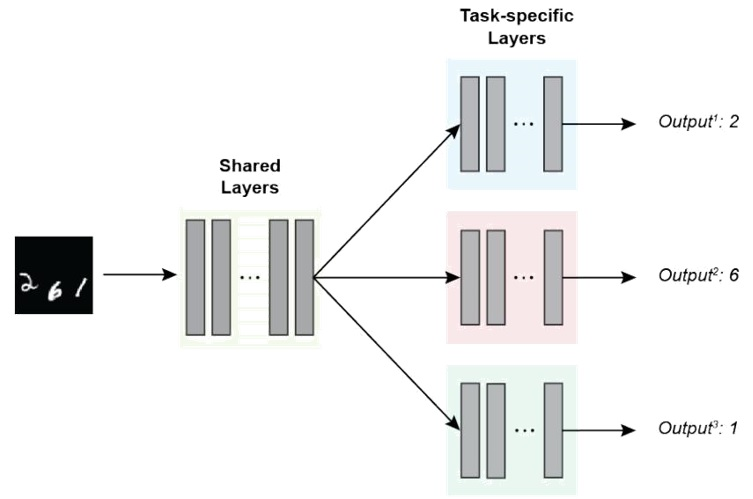
\includegraphics[width=0.7\textwidth]{media/image1.jpg} % Replace with actual path
		\caption{The structure of a conventional hard parameter sharing MTL model.}
		\label{fig:mtl_structure}
	\end{figure}
	
	In order to update the shared layers' weights, the model is supposed to work with one single loss. Regarding this, each task's loss is multiplied by a coefficient indicating the portion of the contribution of that task in the model's learning process. Consequently, choosing these coefficients becomes crucial, especially when the number of tasks is high or there are some kindly contradicting tasks. The significant and difficult nature of the MTL problems due to the large search space has motivated researchers to propose methods that better balance the tasks. In one group of studies \cite{wu2019multi, zhong2019discriminative}, tasks' weights are defined statically and treated as model hyper-parameters so they can be optimized through grid or random search. Although this method is straightforward, it can be impractical for many applications because of its high computational cost. In many other works, an adaptive approach has is used to make a balance between the tasks. GradNorm \cite{chen2018gradnorm} uses the relative inverse training rate to control the learning pace of each task. Similarly, authors in \cite{liu2018end} propose Dynamic Weight Averaging (DWA) that balances the pace at which tasks are performed. It is done by considering the task-specific loss values without the necessity to compute task-specific gradients. Finally, in another category of works, tasks are weighted according to the corresponding uncertainty of tasks. More specifically, in \cite{kendall2018multi}, three tasks of depth regression, semantic, and instance segmentation are balanced according to their homoscedastic uncertainty. The regularization term used in \cite{kendall2018multi} is also used in \cite{liebel2018auxiliary}, but in this work, the positive regularization values are enforced. Moreover, \cite{groenendijk2021multi} presents a new method that benefits from the coefficient of variation to balance multiple tasks.
	
	\section{Uncertainty in nature}
	
	Animals are dealing with a lot of decisions in their daily life, most of which are critical and affect their life. Environmental changes and the existing uncertainties have made this process of decision-making a complicated process for them. Animals, like humans, benefit from a learning mechanism, which helps them to adapt to environmental changes. In other words, they use some learning strategies to cope with environmental uncertainty. In this paper, we categorized these strategies into three main classes based on the time animal poses to make a response.
	
	The first class of strategies includes animals who escape from the sources of uncertainty or unknown factors existing in the environment. In this case, animals have a short time to make a decision. As a result, the next environmental state is not necessarily safe for them \cite{ferrari2018understanding}. For instance, when a prey confronts an unknown species, it has very little time to decide to flee or not.
	
	As the second class of strategies, animals have more time to determine their responses. However, they usually use some estimations about the uncertainty of the environment \cite{schwarz2020how}. The path navigation of ants is a great example of this strategy, i.e., whenever their navigation errors are high and they are too uncertain about their nest location, they adapt their behavior based on three distinct approaches - systematic search, relying on external cues, and Bayesian integration, which are elaborated in subsection \ref{sec:ants_navigation}.
	
	Basically, uncertainty arises from a lack of information from the environment. Based on this fact, in this class of strategies, animals put more time to gain additional information and reduce the uncertainty about the environment \cite{keagy2016female}. Although it is almost analogous to the second strategy, animals gather enough information rather than performing some estimations.
	
	\subsection{Ants navigation}
	\label{sec:ants_navigation}
	
	Like every other animal, ants have to leave their nests to forage. When ants intend to get back to their nest, they merge the directional information available from their path integration (PI) and visual memory \cite{wystrach2015optimal}. PI is a kind of tracking of the environment in each foraging journey. It results in a global vector that continually informs the ant its position and the corresponding relative path to its nest \cite{andel2004path}. It is worth mentioning that relying only on the PI does not necessarily lead the ant to find its nest. This is mainly caused by odor spread affection parameters such as wind speed and hurricane, or by parameters that reflect navigation uncertainty \cite{wolf2005desert}. To deal with these environmental uncertainties, desert ants follow three main strategies which are explained in the following sections.
	
	\subsubsection{Systematic search}
	
	As Tobias Merkle, et al. stated in \cite{merkle2006uncertainty}, by PI, ants acquire a home vector that enables them to return to their nest. However, this does not necessarily lead them to exactly get back to their starting point, in this case, their nest. That is why even small deviations or inaccuracies within the compass will cause a big difference between the assumed position with the actual position. The longer the distance of foraging, the larger the errors occurring. In order to deal with these navigation errors, ants perform a systematic search. The search pattern consists of loops of increasing size centered about the origin \cite{muller1994hidden}, in this case, the position that desert ants assumed is the nest (see Figure \ref{fig:systematic_search}). At regular intervals, they revert to the starting point of the systematic search, in which case, the assumed nest position as calculated by the PI, and then changes the direction in which it turns back next \cite{merkle2006uncertainty}. Algorithm \ref{alg:systematic_search} shows the pseudo-code of the procedure of the systematic search.
	
	\begin{figure}[htbp]
		\centering
		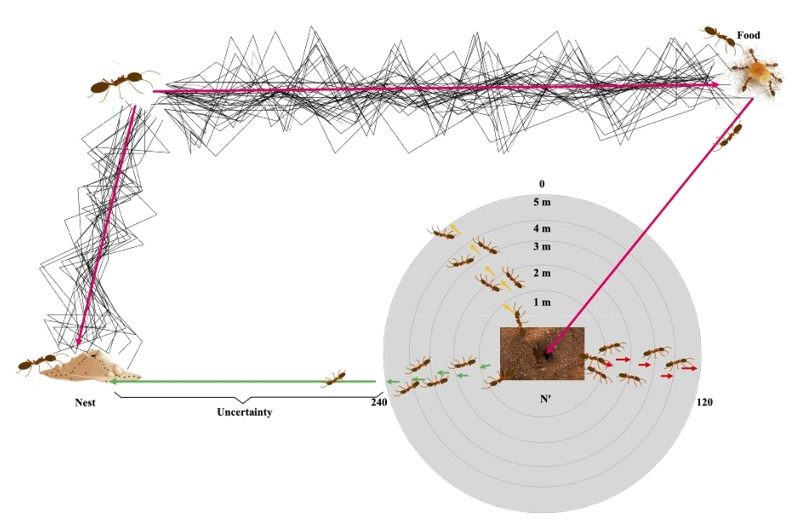
\includegraphics[width=0.7\textwidth]{media/image2.jpg} % Replace with actual path
		\caption{Systematic search consists of loops of increasing size centered about the place where was predicted would be the nest.}
		\label{fig:systematic_search}
	\end{figure}
	
	\begin{algorithm}
		\caption{Pseudo-code for the Systematic Search}
		\label{alg:systematic_search}
		\begin{algorithmic}[1]
			\PROCEDURE{systematicSearch}{position, initialRadius, strideRadius, cutoff}
			\STATE isGoal = GoalCheck(position)
			\STATE radius = initialRadius
			\WHILE{radius $<$ cutoff and not isGoal}
			\STATE isGoal = GoalCheck(position, radius)
			\IF{not isGoal}
			\STATE radius = radius + strideRadius
			\ELSE
			\STATE Move toward the goal
			\ENDIF
			\ENDWHILE
			\ENDPROCEDURE
		\end{algorithmic}
	\end{algorithm}
	
	\subsubsection{Relying on external cues}
	
	This strategy consists of 2 sub-strategies - Error Compensation Strategy (ECS) and Goal Expansion Strategy (GES). Imagine the old seafarers who often would not reach their destination because of existing navigation errors. When traveling to an unknown coast without any particular landmarks, they were not sure which direction to turn. The solution was to steer to one of the sides by a margin exceeding the maximum navigation error to be expected from previous experiences, which is fundamental to ECS. Ants may apply this technique by utilizing the odor as direction to food sources. Directing downwind by an edge fair exceeding the expected maximum route blunder will lead the ants securely over the odor direct and anticipate them from lost indeed little food sources. Let's assume the navigators who could not easily locate the small islands among the vast Pacific ocean relying only on their eyesight. As there were no searching means in that period, they only relied on secondary long-range indicators, for example, birds' behavior or pattern of ocean waves. That is how GES works. By relying on such cues, GES was considerably restricted and the effort to find small islands was significantly reduced. Ants may apply a GES in which using odor as a spatially limited indicator to find the sources of food \cite{wolf2005desert}. Figure \ref{fig:external_cues} pictures the relying on external cues and Algorithm \ref{alg:external_cues} shows a pseudo-code for it.
	
	\begin{figure}[htbp]
		\centering
		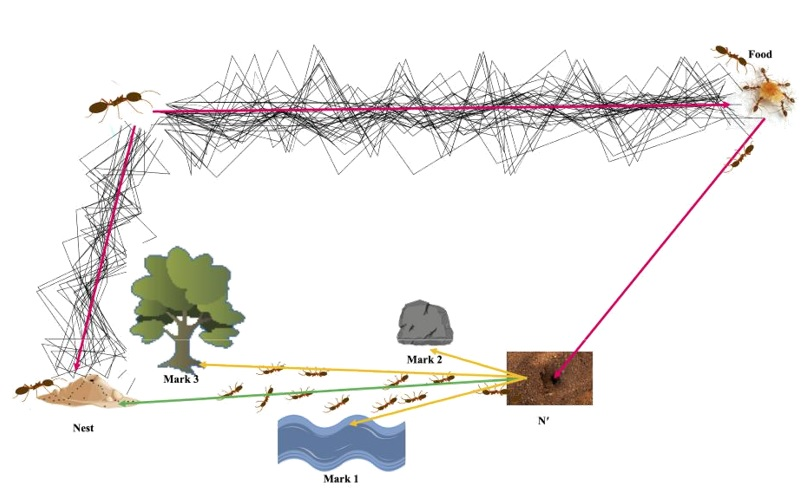
\includegraphics[width=0.7\textwidth]{media/image3.jpg} % Replace with actual path
		\caption{In relying on external cues strategy, ants start to find their nest by relying on various environmental cues.}
		\label{fig:external_cues}
	\end{figure}
	
	\begin{algorithm}
		\caption{Pseudo-code for Relying on External Cues}
		\label{alg:external_cues}
		\begin{algorithmic}[1]
			\PROCEDURE{relyOnExternalCues}{position}
			\STATE currentPosition = position
			\STATE isGoal = GoalCheck(currentPosition)
			\STATE cues = Observe(currentPosition)
			\WHILE{Size(cues) $>$ 0 and not isGoal}
			\STATE cue = GetMostReliableCue(cues)
			\STATE currentPosition = Move(currentPosition, cue)
			\STATE isGoal = GoalCheck(currentPosition)
			\STATE cues = Observe(currentPosition)
			\ENDWHILE
			\ENDPROCEDURE
		\end{algorithmic}
	\end{algorithm}
	
	\subsubsection{Bayesian integration}
	
	All animals follow several cues coming from their instinct and also external sources. However, these cues do not always guide the animal in a unified direction. In other words, they sometimes contradict each other. For instance, to deal with these contradictions, ants trade-off between the external variables and their instinct to navigate their nests. In this approach which is based on Bayesian reasoning, the degree to which each information source contributes to the final decision should be weighted based on the ants' corresponding certainty of that factor \cite{wystrach2015optimal}. That means, for example, if the ants are not familiar with the environment, the weight of the PI vector is relatively greater than the weight of the visual memory vector (see Figure \ref{fig:bayesian_integration}). Moreover, Algorithm \ref{alg:bayesian_integration} shows how Bayesian integration algorithmic works.
	
	\begin{figure}[htbp]
		\centering
		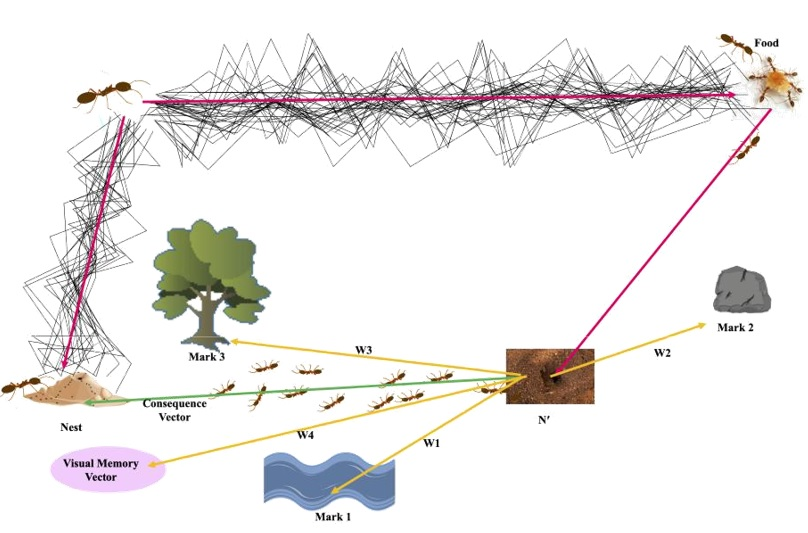
\includegraphics[width=0.7\textwidth]{media/image4.jpg} % Replace with actual path
		\caption{Ants start locating their nest using Bayesian integration by weighting each individual of determinant factors. The weighting process is done based on each individual's corresponding uncertainty.}
		\label{fig:bayesian_integration}
	\end{figure}
	
	\begin{algorithm}
		\caption{Pseudo-code for Bayesian Integration}
		\label{alg:bayesian_integration}
		\begin{algorithmic}[1]
			\PROCEDURE{bayesianIntegration}{position}
			\STATE currentPosition = position
			\STATE isGoal = GoalCheck(currentPosition)
			\STATE cues = Observe(currentPosition)
			\WHILE{Size(cues) $>$ 0 and not isGoal}
			\STATE weights = Weighting(cues)
			\STATE currentPosition = Move(currentPosition, cues, weights)
			\STATE isGoal = GoalCheck(currentPosition)
			\STATE cues = Observe(currentPosition)
			\ENDWHILE
			\ENDPROCEDURE
		\end{algorithmic}
	\end{algorithm}
	
	It is worth mentioning, among all the three aforementioned strategies applied by ants, our proposed method is particularly impressed by the Bayesian integration approach.
	
	\section{Proposed Method}
	
	Consider the training dataset \(X = [x_1, \ldots, x_n]\) with \(n\) samples such that for training sample \(x_i\) the model's prediction is \(\hat{y}_i = [\hat{y}_i^1, \ldots, \hat{y}_i^T]\) where \(T\) denotes the number of the tasks. As in MTL, there is more than one task being evaluated, there is a vector of losses denoted with \(L = [l^1, \ldots, l^T]\) and the total loss is calculated as follows:
	
	\begin{equation}
		l_{\text{total}} = \sum_{i=1}^{T} c^i \cdot l^i
	\end{equation}
	
	where \(l^i\) is the mean loss for task \(i\) and \(c^i\) is its corresponding coefficient. In this paper, we aim to find a set of optimal coefficients leading to minimizing the uncertainty and maximizing the accuracy of the MTL model simultaneously. In this regard, we have found PF a proper mechanism to be used as the foundation of this problem's solution. Additionally, we have found ants' Bayesian integration approach, which reduces their uncertainty of the environment, a great source of inspiration to reduce the prediction uncertainty of the MTL model.
	
	More concretely, given two criteria of performance and uncertainty for evaluating the model, our method seeks to find the best set of weights by which the model's training converges to obtain both an accurate and certain model. In fact, the methodology that we include to consider the tasks' uncertainty in their weighting process is inspired by the ant's Bayesian integration, in which ants weight different cues according to their certainty. Nevertheless, the core idea of converging this weighting strategy to an optimal point is based on PF.
	
	Mathematically, our goal is to obtain the following posterior probability density function (PDF):
	\begin{equation}
		p(C_t | o_{0:t})
		\label{eq:posterior}
	\end{equation}
	where \(C_t = [c^1_t, c^2_t, \ldots, c^T_t]\) is a vector of weights and \(o_{1:t}\) denotes the set of observations that we have already observed until time \(t\). Consequently, since we consider two metrics of performance and uncertainty to evaluate each \(C_t\), each observation itself is a vector of the values obtained according to these two metrics:
	\[
	o_t = \{p_t, u_t\}
	\]
	
	While there are multiple approaches for computing performance and uncertainty, we have computed them as follows:
	\begin{equation}
		p_t = - \sum_{i=1}^{B} \sum_{j=1}^{T} l_{i,t}^j
		\label{eq:performance}
	\end{equation}
	\begin{equation}
		u_t = \text{Variance}(l_{i,t}^j) \quad \forall i \in B
		\label{eq:uncertainty}
	\end{equation}
	where \(l_{i,t}^j\) denotes the computed loss of task \(j\) for batch \(i\) at time \(t\). Moreover, \(B\) represents the number of batches for which each set of weights is evaluated.
	
	We have already formulated our problem. However, the Equation \ref{eq:posterior} cannot be obtained analytically. Therefore, we use an estimation approach to approximate this PDF in which the Equation \ref{eq:posterior} is approximated by a set of particles. However as it is difficult to create the particles directly from this posterior distribution, the following alternative proposal distribution \(\pi(C_t | C_{t-1}^{(i)}, o_{0:t})\) is used for this purpose. Hence, the significance of particle \(i\) is computed using the ratio between the posterior and the proposal distribution, in the following three steps, iteratively:
	
	\begin{itemize}
		\item \textbf{Step 1:} Draw \(N\) particles from the designed distribution:
		\[
		C_t^{(i)} \sim \pi(C_t | C_{t-1}^{(i)}, o_{0:t})
		\]
		
		\item \textbf{Step 2:} Update the particle significance \(q_t^{(i)}\) according to the new observation. The particle significance \(q_t^{(i)}\) are selected using the sampling step which are normalized to satisfy \(\sum_i q_t^{(i)} = 1\).
		\[
		q_t^{(i)} = q_{t-1}^{(i)} \frac{p(o_t | C_t^{(i)}) p(C_t^{(i)} | C_{t-1}^{(i)})}{\pi(C_t^{(i)} | C_{t-1}^{(i)}, o_{0:t})}
		\]
		
		\item \textbf{Step 3:} Go to the re-sampling phase when particle degeneracy happened due to the sampling rate \(R(q_t) = 1 / \sum_i (q_t^{(i)})^2\).
	\end{itemize}
	
	The pseudo-code of our proposed method is shown in the Algorithm \ref{alg:proposed}. \(\text{iter}_{\max}\) is the number of total epochs the model is supposed to be trained for and generate new particles. It is noticeable, the model parameters are not trained separately for the whole number of epochs, rather they are trained for \(\text{iter}_{\text{wu}}\) epochs (called warm-up epochs) and followed by that the initial set of particles is generated. As the warm-up phase finishes, for each mini-batch of \(i\), \(L^t_i\) is computed, and subsequently, \(L_i\) is obtained by multiplying each task's weight, denoted by \(c^t\), by \(L^t_i\). By having \(L_i\), back-propagation and updating the MTL model's parameters occur, respectively. Furthermore, \(\text{iter}_{\text{rs}}\) specifies how often we perform resampling where particles are ranked based on their corresponding observations. Afterward, Gaussian dynamic noise is applied to the \(K\)-best particles to form the next set of particles. In fact, inspired by how ants weight their instincts and environmental landmarks based on Bayesian integration, we combined two uncertainty and performance metrics to evaluate the significance of each particle. More concretely, uncertainty and performance are obtained after applying the tasks' weights found by each particle and evaluating the model's predictions using Equation \ref{eq:performance} and Equation \ref{eq:uncertainty}. Moreover, each particle's significance is the weighted sum of performance and uncertainty, which is inversely related to the dynamic noise variance. In other words, by sampling noise from a Gaussian distribution whose variance is relatively lower, the particles tend to move closer to that selected particle.
	
	\begin{algorithm}
		\caption{Proposed training algorithm}
		\label{alg:proposed}
		\begin{algorithmic}[1]
			\FOR{iter $= 0$ to $\text{iter}_{\max}$}
			\IF{iter $\le$ $\text{iter}_{\text{wu}}$}
			\STATE Warm-up the model's parameters
			\IF{iter $==$ $\text{iter}_{\text{wu}}$}
			\STATE Draw the first particles from initial distribution (Step 1)
			\ENDIF
			\ELSE
			\FOR{i $= 0$ to batchSize}
			\STATE Input batch $x_i$ to compute $L^t_i \ \forall t \in T$
			\STATE Compute $L_i = \sum_{t=1}^{T} c^t L^t_i$
			\IF{i mod evalSize $==$ 0}
			\STATE Store the current particle's observations
			\STATE Load the next particle
			\ENDIF
			\STATE Compute the gradients and backward pass
			\ENDFOR
			\IF{iter mod $\text{iter}_{\text{rs}}$ $==$ 0}
			\STATE Update particles significance (Step 2)
			\STATE Sort particles based on uncertainty and performance combined
			\STATE Choose the $K$-best particles
			\STATE Resample new particles (Step 3)
			\STATE Compute and apply dynamic noise($\sim$ goodness$^{-1}$)
			\STATE Draw next particles (Step 1)
			\ENDIF
			\ENDIF
			\ENDFOR
		\end{algorithmic}
	\end{algorithm}
	
	\section{Experiments}
	
	\subsection{Datasets}
	
	To illustrate the superiority of our method in a more challenging dataset, we evaluated our model on the MTFL dataset containing both regression and classification tasks. In addition, we evaluated our model's functionality on the MultiMNIST dataset.
	
	\subsubsection{MultiMNIST}
	
	MultiMNIST dataset is an extended form of MNIST \cite{deng2012mnist} containing various variations. In the variation that we experimented with, there are 3 digits in each image relying horizontally on each other resulting in 1000 distinct classes. In other words, for this dataset, 3 tasks are supposed to predict the left-digit, middle-digit, and right-digit. To generate the dataset, we used \cite{sun2019multi}. For each class, we use 75 examples, each of which of size 84x84. In this regard, the training set size and the test set size are 48K and 15K, respectively.
	
	The way how each sample is considered is that it is divided into 3 separated labels which will be later used individually as the ground truth for each task (see Figure \ref{fig:multimnist}).
	
	\begin{figure}[htbp]
		\centering
		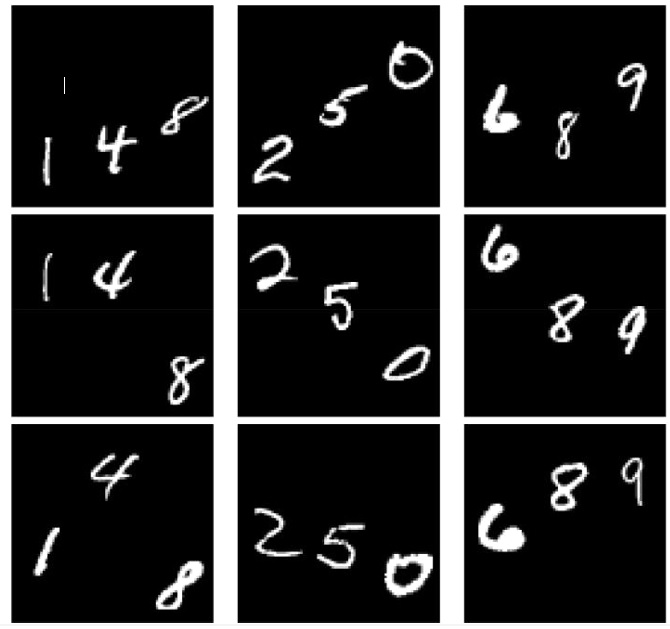
\includegraphics[width=0.6\textwidth]{media/image5.jpg} % Replace with actual path
		\caption{Random samples of 3 different classes of MultiMNIST dataset. The corresponding labels for the left, middle, and right columns are 148, 250, and 689, respectively. The process of preparing labels for the MTL model is that they are first divided into 3 separated labels and then be considered as ground-truth for each task. For instance, the labels of the left column samples will be viewed as \{1, 4, 8\} which are then used as l digit, m digit, and the r digit labels, respectively.}
		\label{fig:multimnist}
	\end{figure}
	
	\subsubsection{The Multi-Task Facial Landmark (MTFL) dataset}
	
	The MTFL dataset \cite{zhang2014facial} contains 12,995 face images. Each image is annotated with five facial landmarks which are the centers of the eyes, nose, and both corners of the mouth. These landmarks will be used for the regression tasks (see Figure \ref{fig:mtfl_samples}). Furthermore, each image contains 4 additional labels associated with the classification tasks. They indicate pose, gender, whether the person is wearing glasses, and whether the person is smiling. For the training and the test phases, we use 10,000 and 2,995 samples, respectively.
	
	\begin{figure}[htbp]
		\centering
		\begin{subfigure}{0.45\textwidth}
			\centering
			\includegraphics[width=\textwidth]{media/image6a.png} % Replace with actual path
			\caption{Random sample 1}
			\label{fig:mtfl_a}
		\end{subfigure}
		\hfill
		\begin{subfigure}{0.45\textwidth}
			\centering
			\includegraphics[width=\textwidth]{media/image6b.png} % Replace with actual path
			\caption{Corresponding output}
			\label{fig:mtfl_b}
		\end{subfigure}
		\par\bigskip
		\begin{subfigure}{0.45\textwidth}
			\centering
			\includegraphics[width=\textwidth]{media/image6c.png} % Replace with actual path
			\caption{Random sample 2}
			\label{fig:mtfl_c}
		\end{subfigure}
		\hfill
		\begin{subfigure}{0.45\textwidth}
			\centering
			\includegraphics[width=\textwidth]{media/image6d.png} % Replace with actual path
			\caption{Corresponding output}
			\label{fig:mtfl_d}
		\end{subfigure}
		\caption{(a) and (c) are two random samples of the MTFL dataset while (b) and (d) are the corresponding output of the MTL model's regression tasks.}
		\label{fig:mtfl_samples}
	\end{figure}
	
	\subsection{Baselines}
	
	To demonstrate the functionality of our proposed method, we compared our results with 4 state-of-the-arts methods results, each of them following a different strategy to find a set of coefficients in an MTL problem. The first one is Uniform Scaling wherein the same coefficients are assigned to each task uniformly. The second baseline is Grad Norm which works based on normalizing the gradients. CoVWeightingLoss is one of the approaches that care about uncertainties and tune the losses based on them. And the last one is Kendall that weights loss functions considering the homoscedastic uncertainty of each task.
	
	\subsection{Training settings}
	
	The network architecture consists of 4 convolutional layers each one followed by batch normalization and maxpooling layer. Following the last maxpooling layer there is a fully-connected layer. These layers form the shared layers of the model. For the task-specific layers, we used two fully connected and one batch normalization layer. It is worth mentioning, for the classification tasks, a softmax layer was used as the model's output layer. Besides, we used ReLU as our non-linear activation function.
	
	The model was trained for 30 and 50 epochs using mini-batches with the size of 256 and 512 on MultiMNIST and MTFL, respectively. We used Adam optimizer \cite{kingma2014adam} with the default parameters explained in the original paper (alpha=0.001, beta1=0.9, beta2=0.999, epsilon=1e-7) for both datasets.
	
	\subsection{Experimental Results}
	
	First, in Table \ref{tab:multimnist_error} we evaluate the methods on the MultiMNIST dataset and report the error obtained for each of the three tasks as well as their average. Our method outperforms all other tasks by a significant margin of 0.32, 0.55, 0.8, and 0.6 for each of those tasks and the average of tasks, respectively. Moreover, to illustrate that our proposed method does not improve the performance at the expense of the uncertainty, we also study the uncertainty in our model's prediction and compare it with the other methods. As shown in Table \ref{tab:multimnist_uncertainty} and Table \ref{tab:multimnist_error}, while our method obtained the least error, i.e. the best performance, it ranked second according to its uncertainty. That means our proposed method is capable of enhancing the prediction accuracy and maintaining the amount of uncertainty at an acceptable level.
	
	\begin{table}[htbp]
		\centering
		\caption{Error on MultiMNIST}
		\label{tab:multimnist_error}
		\begin{tabular}{lcccc}
			\toprule
			Baseline & Left Digit & Middle Digit & Right Digit & Average \\
			\midrule
			Uniform Scaling & 3.76 & 3.41 & 11.24 & 6.14 \\
			Grad Norm & 3.21 & 3.35 & 11.62 & 6.06 \\
			CoVWeightingLoss & 3.68 & 2.90 & 10.68 & 5.75 \\
			Kendall & 3.34 & 2.80 & 10.54 & 5.56 \\
			\textbf{Ours} & \textbf{2.89} & \textbf{2.25} & \textbf{9.74} & \textbf{4.96} \\
			\bottomrule
		\end{tabular}
	\end{table}
	
	\begin{table}[htbp]
		\centering
		\caption{Uncertainty on MultiMNIST}
		\label{tab:multimnist_uncertainty}
		\begin{tabular}{lcccc}
			\toprule
			Baseline & Left Digit & Middle Digit & Right Digit & Average \\
			\midrule
			Uniform Scaling & 0.58 & 0.58 & 0.25 & 0.45 \\
			Grad Norm & 0.46 & 0.51 & 0.29 & 0.41 \\
			CoVWeightingLoss & 0.55 & 0.56 & 0.22 & 0.42 \\
			Kendall & 0.44 & 0.45 & 0.21 & 0.35 \\
			\textbf{Ours} & \textbf{0.50} & \textbf{0.46} & \textbf{0.27} & \textbf{0.40} \\
			\bottomrule
		\end{tabular}
	\end{table}
	
	Furthermore, we also compare the performance and uncertainty of models in a quite larger dataset, MTFL. Table \ref{tab:mtfl_error} illustrates the overall result of models' performance evaluation. Our method obtains the least regression error in four tasks out of five, and on average it significantly outperforms other methods. Similarly, in classification tasks, our method considerably performs better than the other ones on average and it achieves the least classification error, 0.98. Moreover, despite the impressive performance gained by our method in the above evaluation, the most important part of our experiments is shown in Table \ref{tab:mtfl_uncertainty}, where different methods are compared according to their prediction uncertainty. As illustrated, our method shows very competitive uncertainty with other methods, even those directly aim at reducing the uncertainty. More precisely, it obtains the second least uncertainty in average among regression tasks, and the least uncertainty between classification ones, by a noticeable margin of 0.64. This together with the competence of our method to reach high performance, implies the efficiency of our method for the applications wherein uncertainty is also important besides the model's performance.
	
	\begin{table}[htbp]
		\centering
		\caption{The MTFL multi-task error per attribute for all algorithms.}
		\label{tab:mtfl_error}
		\begin{tabular}{lccccccccccc}
			\toprule
			& \multicolumn{5}{c}{Regression} & & \multicolumn{4}{c}{Classification} & \\
			\cmidrule(lr){2-6} \cmidrule(lr){8-11}
			Baseline & Left eye & Right eye & Nose & Left mouth corner & Right mouth corner & Average & & Gender & Smile & Glasses & Pose & Average \\
			\midrule
			Uniform Scaling & 19.81 & 9.54 & 11.30 & 10.89 & 6.00 & 11.51 & & 2.57 & 1.60 & 1.37 & 0.60 & 1.54 \\
			CoVWeightingLoss & 12.12 & 7.72 & 9.85 & 6.40 & 5.60 & 8.34 & & 2.27 & 4.41 & 0.33 & 0.73 & 1.94 \\
			Grad Norm & 8.81 & 6.41 & 6.87 & 8.01 & 5.75 & 7.17 & & 2.49 & 0.56 & 0.45 & 1.10 & 1.15 \\
			Kendal et al. & 12.95 & 9.40 & 10.01 & 10.76 & 10.24 & 10.67 & & 3.71 & 0.97 & 1.21 & 0.74 & 1.66 \\
			\textbf{Ours} & \textbf{7.01} & \textbf{6.80} & \textbf{5.79} & \textbf{6.24} & \textbf{5.39} & \textbf{6.25} & & \textbf{0.93} & \textbf{0.70} & \textbf{0.63} & \textbf{1.66} & \textbf{0.98} \\
			\bottomrule
		\end{tabular}
	\end{table}
	
	\begin{table}[htbp]
		\centering
		\caption{The MTFL multi-task uncertainty per attribute for all algorithms (uncertainty $\times 100$).}
		\label{tab:mtfl_uncertainty}
		\begin{tabular}{lccccccccccc}
			\toprule
			& \multicolumn{5}{c}{Regression} & & \multicolumn{4}{c}{Classification} & \\
			\cmidrule(lr){2-6} \cmidrule(lr){8-11}
			Baseline & Left eye & Right eye & Nose & Left mouth corner & Right mouth corner & Average & & Gender & Smile & Glasses & Pose & Average \\
			\midrule
			Uniform Scaling & 5.20 & 4.75 & 4.66 & 5.07 & 4.82 & 4.90 & & 4.08 & 3.96 & 3.53 & 2.81 & 3.59 \\
			CoVWeightingLoss & 4.08 & 4.43 & 5.87 & 3.98 & 4.01 & 4.48 & & 3.49 & 17.89 & 1.54 & 3.35 & 6.57 \\
			Grad norm & 4.59 & 4.75 & 5.39 & 5.25 & 5.12 & 5.02 & & 4.41 & 2.56 & 1.65 & 3.47 & 3.02 \\
			Kendal et al. & 4.27 & 4.48 & 4.95 & 5.02 & 5.18 & 4.78 & & 7.51 & 3.87 & 3.53 & 6.18 & 5.27 \\
			\textbf{Ours} & \textbf{4.25} & \textbf{4.89} & \textbf{4.03} & \textbf{5.00} & \textbf{5.25} & \textbf{4.68} & & \textbf{2.16} & \textbf{1.62} & \textbf{1.78} & \textbf{3.97} & \textbf{2.38} \\
			\bottomrule
		\end{tabular}
	\end{table}
	
	To illustrate the efficiency of the PF algorithm in terms of finding optimal points, we first designed a simplified intuitive experiment (see Figure \ref{fig:particle_motion}) and then extended the observation to MTFL and MultiMNIST datasets (see Figure \ref{fig:particles_multimnist} and Figure \ref{fig:particles_mtfl}). In the first experiment, we plotted a random one-dimensional curve containing several local minimums as well as a global one that is the target point. We then employed the PF algorithm to find this point. Consequently, as the first step of the algorithm, some random particles are generated, and then, iteratively, based on the proficiency of particles, the next set of particles is produced. As the figure illustrates, the process of randomly generating particles would help the algorithm to explore different points as well as escape the sub-optimal solutions.
	
	\begin{figure}[htbp]
		\centering
		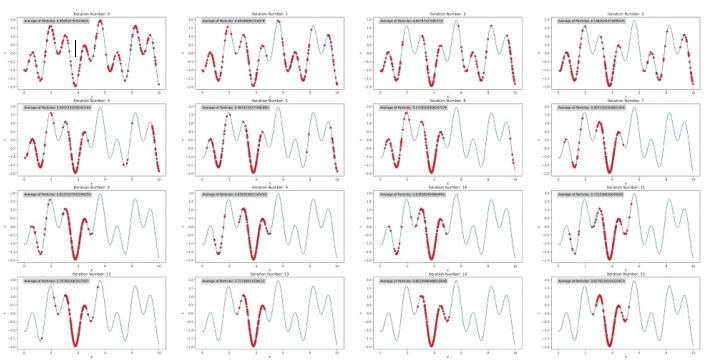
\includegraphics[width=0.8\textwidth]{media/image7.jpg} % Replace with actual path
		\caption{Here the motion of particles through an 1-dimensional function in order to meet the global minimum is illustrated. As the first step, particles are distributed randomly over the search space. Through the next iterations, as the next set of particles is produced, they tend to gradually converge to the subspace that seems more promising in terms of having the minimum value.}
		\label{fig:particle_motion}
	\end{figure}
	
	Having successfully applied the PF algorithm to the above-mentioned problem, we then designed a similar experiment on two MTFL and MultiMNIST datasets. However, to overcome the problem of visualization in high dimensional data, we used a visualization technique, called Star Coordinates \cite{kandogan2000star}. It arranges the coordinate axes with equal angles between them on a circle that is on a two-dimensional plane, and all data points are scaled to the length of the axis. Therefore, each two-dimensional point in the Figure \ref{fig:particles_multimnist} and Figure \ref{fig:particles_mtfl} represents a three and nine-dimensional set of tasks' weights respectively, by which the multi-task model has been trained. Subsequently, after performing our method for 8 steps, we plotted the average point of each generation along with its corresponding radius showing the generation's diversity. Finally, to demonstrate the superiority of the final points over the starting points, we separately trained the MTL model for both datasets with the tasks' weights equal to the weights of starting and ending points. The results can be seen in Table \ref{tab:nest_comparison_multimnist} and Table \ref{tab:nest_comparison_mtfl} where they both demonstrate that the ending points in both datasets contain the weights which lead to a model with higher performance and lower uncertainty. Therefore, starting from initial random weights, our proposed method is capable of improving the quality of weights in terms of both performance and uncertainty.
	
	\begin{figure}[htbp]
		\centering
		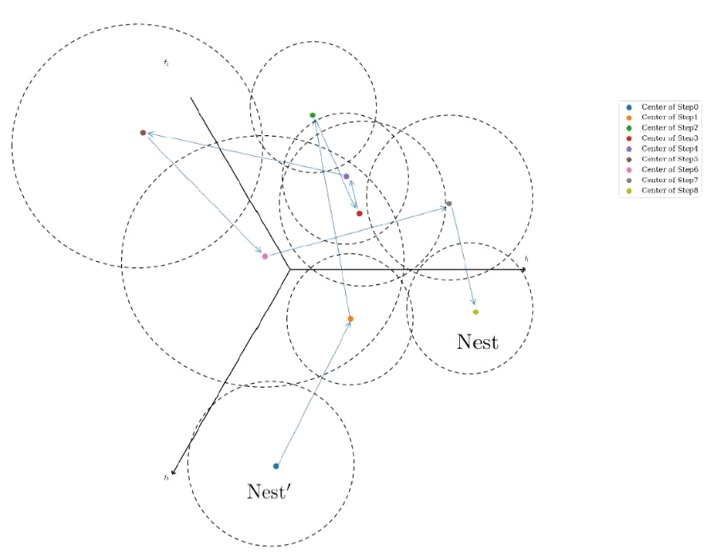
\includegraphics[width=0.8\textwidth]{media/image8.jpg} % Replace with actual path
		\caption{Illustration of the particles' moving during training of an MTL model on Multi-MNIST dataset.}
		\label{fig:particles_multimnist}
	\end{figure}
	
	\begin{figure}[htbp]
		\centering
		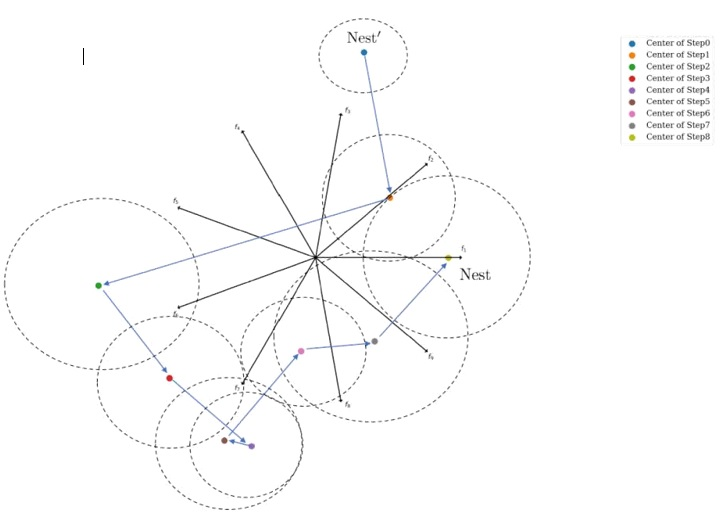
\includegraphics[width=0.8\textwidth]{media/image9.jpg} % Replace with actual path
		\caption{Illustration of the particles' moving during training of an MTL model on MTFL dataset.}
		\label{fig:particles_mtfl}
	\end{figure}
	
	\begin{table}[htbp]
		\centering
		\caption{Comparison of performance and uncertainty of two Nest' and Nest on MultiMNIST}
		\label{tab:nest_comparison_multimnist}
		\begin{tabular}{lcc}
			\toprule
			Point & Performance & Uncertainty \\
			\midrule
			Nest' & 6.57 & 0.53 \\
			Nest & 5.95 & 0.47 \\
			\bottomrule
		\end{tabular}
	\end{table}
	
	\begin{table}[htbp]
		\centering
		\caption{Comparison of performance and uncertainty of two Nest' and Nest on MTFL dataset}
		\label{tab:nest_comparison_mtfl}
		\begin{tabular}{lcc}
			\toprule
			Point & Performance & Uncertainty \\
			\midrule
			Nest' & 1.57 & 3.92 \\
			Nest & 1.10 & 2.92 \\
			\bottomrule
		\end{tabular}
	\end{table}
	
	\section{Conclusion and future works}
	
	We proposed a method for finding a set of optimal coefficients in order to solve MTL problems. More concretely, the set of optimal coefficients causes a DNN model with high performance and a low level of uncertainty simultaneously. Our proposed method benefited from PF and was mainly inspired by how ants cope with navigation uncertainties. Generally, ants use different approaches to navigate to their nests while there are environmental uncertainties. We brought the insight we found from ants' Bayesian integration into the field of DNNs by drawing noises from a dynamic-variance Gaussian distribution. Moreover, inspired by that we combined two metrics for evaluating and training the MTL model. Comparing the results discussed in subsection 5.4, we demonstrated that our proposed method adequated achieving a low level of uncertainty without considerably harming the model performance. Furthermore, for future works we consider doing as follows:
	
	\begin{itemize}
		\item Among the several ant navigation approaches, discussed in subsection 3.1, we only used one of them for training DNNs. However, we hope to be able to take advantage of the other approaches as well in future works.
		\item As mentioned in section 3 animals' reactions while facing uncertainty can be categorized into 3 classes, based on how much time they have to respond to the stimulus. We believe that we can take advantage of this categorization in trend topics of DNNs learning, such as Online learning.
		\item Since our proposed method is highly reproducible and demands insignificant changes in the training process, we can also easily use this method in order to find other hyperparameters, particularly, in cases that more than one measurement metric is supposed to be used.
	\end{itemize}
	
	\section*{Acknowledgments}
	We would especially like to thank Tahereh Bahraini who was by our side, helped us with illustrations, and provided us with instructive information about PF.
	
	\bibliographystyle{plain}
	\begin{thebibliography}{99}
		
		\bibitem{castiglioni2021ai}
		I. Castiglioni, L. Rundo, M. Codari, G. Di Leo, C. Salvatore, M. Interlenghi, F. Gallivanone, A. Cozzi, N. C. D'Amico, F. Sardanelli, Ai applications to medical images: From machine learning to deep learning, Physica Medica 83 (2021) 9--24.
		
		\bibitem{aggarwal2021diagnostic}
		R. Aggarwal, V. Sounderajah, G. Martin, D. S. Ting, A. Karthikesalingam, D. King, H. Ashrafian, A. Darzi, Diagnostic accuracy of deep learning in medical imaging: A systematic review and meta-analysis, NPJ digital medicine 4 (1) (2021) 1--23.
		
		\bibitem{fischer2018deep}
		T. Fischer, C. Krauss, Deep learning with long short-term memory networks for financial market predictions, European Journal of Operational Research 270 (2) (2018) 654--669.
		
		\bibitem{kamara2022ensemble}
		A. F. Kamara, E. Chen, Z. Pan, An ensemble of a boosted hybrid of deep learning models and technical analysis for forecasting stock prices., Information Sciences (2022).
		
		\bibitem{caruana1997multitask}
		R. Caruana, Multitask learning, Machine learning 28 (1) (1997) 41--75.
		
		\bibitem{zheng2020discriminative}
		H. Zheng, R. Wang, W. Ji, M. Zong, W. K. Wong, Z. Lai, H. Lv, Discriminative deep multi-task learning for facial expression recognition, Information Sciences 533 (2020) 60--71.
		
		\bibitem{chen2018multi}
		Y. Chen, D. Zhao, L. Lv, Q. Zhang, Multi-task learning for dangerous object detection in autonomous driving, Information Sciences 432 (2018) 559--571.
		
		\bibitem{hossin2015review}
		M. Hossin, M. N. Sulaiman, A review on evaluation metrics for data classification evaluations, International journal of data mining \& knowledge management process 5 (2) (2015) 1.
		
		\bibitem{sefati2017towards}
		M. Sefati, J. Chandiramani, K. Kreisköther, A. Kampker, S. Baldi, Towards tactical behaviour planning under uncertainties for automated vehicles in urban scenarios, in: 2017 IEEE 20th International Conference on Intelligent Transportation Systems (ITSC), IEEE, 2017, pp. 1--7.
		
		\bibitem{ayhan2020expert}
		M. S. Ayhan, L. Kühlewein, G. Aliyeva, W. Inhoffen, F. Ziemssen, P. Berens, Expert-validated estimation of diagnostic uncertainty for deep neural networks in diabetic retinopathy detection, Medical Image Analysis 64 (2020) 101724.
		
		\bibitem{delmoral1997nonlinear}
		P. Del Moral, Nonlinear filtering: Interacting particle resolution, Comptes Rendus de l'Académie des Sciences-Series I-Mathematics 325 (6) (1997) 653--658.
		
		\bibitem{botvinick2019reinforcement}
		M. Botvinick, S. Ritter, J. X. Wang, Z. Kurth-Nelson, C. Blundell, D. Hassabis, Reinforcement learning, fast and slow, Trends in cognitive sciences 23 (5) (2019) 408--422.
		
		\bibitem{ruder2017overview}
		S. Ruder, An overview of multi-task learning in deep neural networks, arXiv preprint arXiv:1706.05098 (2017).
		
		\bibitem{wu2019multi}
		H. Wu, M. Xin, W. Fang, H. M. Hu, Z. Hu, Multi-Level Feature Network with Multi-Loss for Person Re-Identification, IEEE Access 7 (2019) 91052--91062.
		
		\bibitem{zhong2019discriminative}
		W. Zhong, T. Zhang, L. Jiang, J. Ji, Z. Zhang, H. Xiong, Discriminative representation learning for person re-identification via multi-loss training, Journal of Visual Communication and Image Representation 62 (2019) 267--278.
		
		\bibitem{chen2018gradnorm}
		Z. Chen, V. Badrinarayanan, C. Y. Lee, A. Rabinovich, GradNorm: Gradient normalization for adaptive loss balancing in deep multitask networks, arXiv (2017).
		
		\bibitem{liu2018end}
		S. Liu, E. Johns, A. J. Davison, End-to-end multi-task learning with attention, arXiv (2018).
		
		\bibitem{kendall2018multi}
		A. Kendall, Y. Gal, R. Cipolla, Multi-task learning using uncertainty to weigh losses for scene geometry and semantics, in: Proceedings of the IEEE conference on computer vision and pattern recognition, 2018, pp. 7482--7491.
		
		\bibitem{liebel2018auxiliary}
		L. Liebel, M. Körner, Auxiliary tasks in multi-task learning, arXiv preprint arXiv:1805.06334 (2018).
		
		\bibitem{groenendijk2021multi}
		R. Groenendijk, S. Karaoglu, T. Gevers, T. Mensink, Multi-loss weighting with coefficient of variations, in: Proceedings of the IEEE/CVF Winter Conference on Applications of Computer Vision, 2021, pp. 1469--1478.
		
		\bibitem{ferrari2018understanding}
		M. C. Ferrari, G. E. Brown, D. P. Chivers, Understanding the effect of uncertainty on the development of neophobic antipredator phenotypes, Animal Behaviour 136 (2018) 101--106.
		
		\bibitem{schwarz2020how}
		S. Schwarz, L. Clement, E. Gkanias, A. Wystrach, How do backward-walking ants (cataglyphis velox) cope with navigational uncertainty?, Animal Behaviour 164 (2020) 133--142.
		
		\bibitem{keagy2016female}
		J. Keagy, L. C. Hosler, G. Borgia, Female active sampling of male paint on bowers predicts female uncertainty in mate choice, Animal Behaviour 116 (2016) 131--137.
		
		\bibitem{wystrach2015optimal}
		A. Wystrach, M. Mangan, B. Webb, Optimal cue integration in ants, Proceedings of the Royal Society B: Biological Sciences 282 (1816) (2015) 20151484.
		
		\bibitem{andel2004path}
		D. Andel, R. Wehner, Path integration in desert ants, cataglyphis: how to make a homing ant run away from home, Proceedings of the Royal Society of London. Series B: Biological Sciences 271 (1547) (2004) 1485--1489.
		
		\bibitem{wolf2005desert}
		H. Wolf, R. Wehner, Desert ants compensate for navigation uncertainty, Journal of Experimental Biology 208 (22) (2005) 4223--4230.
		
		\bibitem{merkle2006uncertainty}
		T. Merkle, M. Knaden, R. Wehner, Uncertainty about nest position influences systematic search strategies in desert ants, Journal of Experimental Biology 209 (18) (2006) 3545--3549.
		
		\bibitem{muller1994hidden}
		M. Müller, R. Wehner, The hidden spiral: systematic search and path integration in desert ants, cataglyphis fortis, Journal of Comparative Physiology A 175 (5) (1994) 525--530.
		
		\bibitem{deng2012mnist}
		L. Deng, The mnist database of handwritten digit images for machine learning research, IEEE Signal Processing Magazine 29 (6) (2012) 141--142.
		
		\bibitem{sun2019multi}
		S.-H. Sun, Multi-digit mnist for few-shot learning (2019).
		URL \url{https://github.com/shaohua0116/MultiDigitMNIST}
		
		\bibitem{zhang2014facial}
		Z. Zhang, P. Luo, C. C. Loy, X. Tang, Facial landmark detection by deep multi-task learning, in: European conference on computer vision, Springer, 2014, pp. 94--108.
		
		\bibitem{kingma2014adam}
		D. P. Kingma, J. Ba, Adam: A method for stochastic optimization, arXiv preprint arXiv:1412.6980 (2014).
		
		\bibitem{kandogan2000star}
		E. Kandogan, Star coordinates: A multi-dimensional visualization technique with uniform treatment of dimensions, in: Proceedings of the IEEE information visualization symposium, Vol. 650, Citeseer, 2000, p. 22.
		
	\end{thebibliography}
	
\end{document}